% Created 2019-12-02 Mon 15:44
% Intended LaTeX compiler: pdflatex
\documentclass[11pt]{article}
\usepackage[utf8]{inputenc}
\usepackage[T1]{fontenc}
\usepackage{graphicx}
\usepackage{grffile}
\usepackage{longtable}
\usepackage{wrapfig}
\usepackage{rotating}
\usepackage[normalem]{ulem}
\usepackage{amsmath}
\usepackage{textcomp}
\usepackage{amssymb}
\usepackage{capt-of}
\usepackage{hyperref}
\usepackage{color}
\usepackage{listings}
\usepackage{setspace}
\doublespacing
\usepackage[citestyle=authoryear,bibstyle=authortitle,hyperref=true,backref=true,maxcitenames=3,uniquename=false,maxbibnames=99,url=true,backend=biber,natbib=true] {biblatex}
\usepackage[margin=1in]{geometry}
\usepackage{array}
\newcolumntype{C}[1]{>{\centering\arraybackslash}p{#1}}
%\ExecuteBibliographyOptions{parentracker=false}
\makeatletter
\newrobustcmd*{\parentexttrack}[1]{%
\begingroup
\blx@blxinit
\blx@setsfcodes
\blx@bibopenparen#1\blx@bibcloseparen
\endgroup}
\AtEveryCite{%
\let\parentext=\parentexttrack%
\let\bibopenparen=\bibopenbracket%
\let\bibcloseparen=\bibclosebracket}
\makeatother
\addbibresource{/home/matt/Dropbox/BibLaTeX/library.bib}
\author{Matt DeAngelis}
\date{\today}
\title{}
\hypersetup{
 pdfauthor={Matt DeAngelis},
 pdftitle={},
 pdfkeywords={},
 pdfsubject={},
 pdfcreator={Emacs 26.3 (Org mode 9.1.9)}, 
 pdflang={English}}
\begin{document}

\begin{titlepage}
\singlespacing
\begin{center}
\LARGE Sympathy for the Noise Trader: Limitations of Learning from Price
\vspace*{35mm}

\normalsize Matthew D. DeAngelis\textsuperscript{a}

\textit{Georgia State University}
\end{center}

\vspace*{\fill}
\textsuperscript{a} Corresponding author. School of Accountancy, J. Mack Robinson College of Business, Georgia State University, 35 Broad Street, Room 512, Atlanta GA, 30302. Phone: (404) 413-7214. E-mail: mdeangelis@gsu.edu

\vspace*{10mm}
I gratefully acknowledge the contributions of Kris Allee, John Campbell, Vic Lee, Ruiyan Luo, Joao Mota, Greg Waymire, James Wilhelm, Jing Zhang and Lu Zhang. 
\end{titlepage}

\newpage

\begin{center}
\LARGE Sympathy for the Noise Trader: Limitations of Learning from Price
\end{center}
\vspace*{40mm}
\begin{abstract}


Empirical studies in accounting and finance assume that the market not only incorporates all available information into price, but also forms precise and efficient estimates of individual valuation parameters such as the persistence of earnings. However, prevailing models of investor learning do not provide a mechanism by which investors distinguish between multiple parameters when observing aggregate price movements. I extend the model in \citet{grossmanImpossibilityInformationallyEfficient1980} to accommodate multiple parameters and find that the market prices aggregate \textbf{all} information efficiently but do not achieve efficient estimates of \textbf{individual parameters}. As a result, it is not clear that researchers can claim that the market estimates these parameters. My study asks whether the literature ascribes too much power to price in communicating information between investors.
\end{abstract}
\newpage

\section{Introduction}
\label{sec:org21e97a0}
In this paper, I explore the limitations of learning from price. Specifically, I extend previous models of investor learning to accommodate the simultaneous processing of multiple information signals. Prior models focus on learning from price as a perfect or noisy signal for a single informational parameter (\citet{grossmanImpossibilityInformationallyEfficient1980,diamondInformationAggregationNoisy1981}). However, in practice information rarely arrives in isolation: detailed numerical or textual information can be released as part of an earnings announcement; managers can issue a forecast in conjunction with earnings; and an annual report can contain hundreds of pages. I investigate what happens when uninformed investors must revise their estimates of multiple valuation parameters from movements in a single price signal. 

Following \citet{grossmanImpossibilityInformationallyEfficient1980} (GS), I create an agent-based simulation to model the process of uninformed investors learning private information from informed investors. Specifically, I create informed agents with perfect knowledge of a single informational parameter and uninformed agents that must learn that parameter by observing the price signal. Consistent with GS, I find that the market converges on the ``true'' price of the security and that uninformed investors arrive at an accurate estimate of the parameter. 

Also consistent with GS, I find that the market continues to converge to the true value of the security when I extend the security to include two informational parameters. In this sense, the market is efficient in that the price impounds all available information. However, the market's information set is neither complete nor accurate: the consensus estimate of the individual parameters across individual traders does not converge on the true value of those parameters. This is because uninformed traders cannot distinguish the values of the individual parameters from the aggregate price movement. Instead, they approximate a linear combination of the parameters that is consistent with the observed price. As such, whether market price aggregates \textbf{all} available information is distinct from whether the market learns \textbf{each component} of information. I also find evidence to suggest that investors learn individual parameters less well as the number of parameters grows beyond two.

I make two primary contributions to the literature. First, although empirical researchers often refer to a cognitive model of the market, in which the market ``learns'' or ``estimates'' the value of a security and its components, a precise model of what the market ``knows'', and how, is not specified. Further, many studies appear to assume that an efficient price implies an efficient valuation of each individual parameter that makes up price, or that investors learn specifically what weight to assign to current earnings, detailed balance sheet information, linguistic tone, etc., from price movements around earnings releases. Since the market only maintains a single informational item, price, that is distinct from the models held by individual investors, I ask whether the market can be said to ``know'' value beyond price. I find that the market can converge upon the correct price of a security without establishing a correct consensus estimate on the individual parameters of value. This result is consistent with what empirical researchers have long acknowledged regarding their own limitations in separating the price impact of multiple signals. However, market models do not incorporate these limitations when modeling investor learning. In clarifying this disconnect between theory and empirical practice, my study helps to explain empirical evidence of price drift after significant information releases such as earnings, as well as a habit by investors to collect and respond to so-called ``stale'' information (\citet{tetlockAllNewsThat2011,drakeUsefulnessHistoricalAccounting2016a}). It also questions the assumption that the market should only respond to ``surprises'' in parameters, which would indicate that the market has efficiently priced each realization of the parameter prior to subsequent realizations.

Second, I highlight the utility of simulations to explore theoretical questions in accounting research. Simulations provide an opportunity to examine complex systems in which behavior is unpredictable and dependent on interactions between agents (\citet{lebaronAgentbasedComputationalFinance2000}). They also provide an intuitive way to construct and experiment with analytical models and to make those models accessible to empirical researchers. In the spirit of reproducible research, I provide all of the code used in this study directly in the paper so that editors, reviewers and future researchers can replicate, stress-test and extend my results. My code is written in a Lisp dialect, Clojure, which makes it easy to modify and extend to new models and experiments for investigating investor and market information processing. I ask that researchers utilizing this code also open source their modifications to encourage collaboration, save researcher time, and improve understanding of how researcher choices influence results.

\section{Literature Review and Hypothesis Development}
\label{sec:orga9be873}
\subsection{Learning from price}
\label{sec:orgfb6dcb7}
What precisely is meant by market efficiency, as well as what and how investors learn from price, is usually not specified in empirical studies. However, a discussion in \citet{tetlockGivingContentInvestor2007}, regarding how the market is expected to respond to the release of media articles, is instructive as to the assumptions commonly made.

\citet{tetlockGivingContentInvestor2007} considers how the market is expected to respond under three alternative situations:
\begin{enumerate}
\item Media articles convey new information to the market. In this case, the market price is expected to adjust and this adjustment is expected to persist.
\item Media articles convey old information to the market. In this case, the market price is not expected to adjust, since the information is already incorporated in price.
\item Media articles reflect ``sentiment'' in the market. In this case, the market price is expected to adjust, but this adjustment is expected to reverse as arbitrageurs trade back to fundamentals.
\end{enumerate}
Each alternative requires that investors not only know price, but know why price is what it is. How else would an investor distinguish between old information and new information, if he is not able to observe price and infer the information contained within it? Likewise with sentiment: an investor must understand whether private information exists and whether price incorporates that information before concluding that an observed price movement has no informational basis. A similar set of assumptions is commonly used in the accounting literature. In \citet{kormendiEarningsInnovationsEarnings1987}, for example: ``Implicit in [Equation] 1 is the efficient markets assumption that only the new information in earnings affects returns.'' (page 326). This suggests that the market develops an efficient estimate, not just of the total information available to value the security, but of earnings specifically. Moreover, while Kormendi and Lipe make this assumption over an entire year's time, subsequent studies use an event-study framework in which the market is presumed to fully price earnings within a few days, or even hours. In other words, investors are presumed to exit the trading process with a correct estimate of the weight to assign to earnings, at least on average, so that future price movements are determined only by earnings innovations. 

These assumptions regarding investor and market learning are based on models showing price to be a powerful information communicator, of which \citet{grossmanImpossibilityInformationallyEfficient1980} (GS) is one of the most prominent. GS utilize a market model in which the return from a single risky security is based on a single informational parameter, so that return is represented as:
\begin{equation}
u = \theta + \epsilon
\end{equation}
where \(\theta\) represents the mean of the return distribution. Investors can purchase \(\theta\) and become informed investors. Otherwise, uninformed investors can learn \(\theta\) through price movements. 

GS' main finding is that price can be too informative: it communicates the valuation parameter so well that it creates a disincentive for investors to become informed. Specifically, because the benefits of becoming informed decline as more investors become informed, communication of information through price reduces the likelihood that the marginal investor chooses to purchase information. In order for the market to reach equilibrium, GS finds that market prices must convey \(\theta\) with noise so that returns to information gathering are more stable.

Price can become a sufficient statistic for unobservable information even in the absence of fully informed investors. In \citet{grossmanEfficiencyCompetitiveStock1976}, \citet{diamondInformationAggregationNoisy1981}, and \citet{verrecchiaConsensusBeliefsInformation1980}, investors are either endowed with or can purchase random draws from the return variable, so that no individual investor knows the true mean of returns. However, their collective information converges on the true mean, again allowing individual investors to rely solely on price and discouraging them from collecting information. As above, in order for markets to function, price must be made less informative or, as noted in Diamond and Verrecchia, ``[n]oise is critical to the analysis of the model’s equilibrium'' (page 233). This noise ``represents factors other than information which cause prices to vary'' (page 234), allowing informed investors to profit from information gathering.

Other models of noisy investor learning include \citet{brayLearningEstimationStability1982} and \citet{brayRationalExpectationsEquilibria1986}, in which investors must learn to form rational expectations from price because the relationship between price and the security's underlying value changes over time. In these models investors use econometric models such as linear regression to estimate this relationship. \citet{fourgeaudLearningProceduresConvergence1986} allow decision-makers to predict an unobservable endogenous factor from observable exogenous factors. In each of these cases, however, investors tie a single price to a single information parameter.

As pointed out in \citet{verrecchiaConsensusBeliefsInformation1980}, the market can be said to have learned the distribution of value even if all investors do not agree. Instead, investors could be dispersed around the true mean on the univariate prior. The disagreement around the prior results in trading, but the same number of investors revise their beliefs upwards as downwards, in the same amounts. In this case there is trading, at least for a time, but the trading results in no price movement. In both cases, however, the market can be said to have reached both an efficient estimate of price, or the total value of the security, as well as each of the components of value (since there is only a single component). 

Models that do consider multiple information parameters combine them with multiple prices. Usually this constitutes a simulation of an entire market in which investors trade across multiple securities in an effort to achieve an efficient price equilibrium.  \citet{blumeLearningBeRational1982} is a notable early contribution to this literature, along with studies such as \citet{axtellComplexityExchange2005} that explore the utility of different trading mechanisms. However, the ratio of parameters to prices in these models remains one-to-one: \citet{blumeLearningBeRational1982} specifically indicate that signals and prices must be paired in order for their model of Bayesian learning to function (pages 343-344). As such, these models do not extend to situations where price is determined by more than one valuation parameter: since there is a one-to-one mapping between the underlying parameter and price, it is trivial for an investor to determine whether price conveys new information and how to incorporate that information into her own estimate. If the price an investor observes is consistent with her univariate prior, she rightly believes that she has learned all that she needs to know. A media article reaffirming that belief has no affect on her trading. 

However, it is not clear that this pattern extends to a multivariate prior. If there are multiple combined values of parameters that can lead to the same price, then investors 1) cannot perfectly infer from price movements which parameter requires revision and 2) cannot perfectly infer from information about parameters what the price response should be. As a result, price no longer conveys perfect information and no longer requires the introduction of noise to prevent perfect learning.

\section{Model}
\label{sec:org7ef693a}
I begin by constructing an agent-based market simulation to reproduce the model of investor learning in \citet{grossmanImpossibilityInformationallyEfficient1980} (GS). I start with GS because their model contains a single valuation parameter that uninformed investors can learn solely through price. It is not my intention to perfectly replicate GS' model, but rather to create a similar set of circumstances for investor learning.

Following GS, I create two types of investor. One type of investor is fully informed, the other uninformed. Operationally, this means that a fully informed investor's prior is equal to the true value of the security. An uninformed investor's prior consists of a random draw from a normal distribution. The following function creates either an informed or uninformed investor, depending on its arguments:

\singlespacing
\lstset{language=Lisp,label= ,caption= ,captionpos=b,numbers=none}
\begin{lstlisting}
(defn make-investor
  ([n] ;; Makes an uninformed agent
   {:prior (vec (repeatedly n (fn [] {:informed? false :value (draw-round)}))) 
    :id (uuid)})
  ([v fully?] ;; Makes an informed agent from a vector of parameters
   {:prior
    (if fully?
      (mapv (fn [pr] {:informed? true :value pr}) v)
      (let [i (rand-int (count v))]
        (assoc (:prior (make-investor (count v)))
               i
               {:informed? true :value (get v i)})
        ))
    :id (uuid)})
  )
\end{lstlisting}
\doublespacing

See \hyperref[sec:org95e66fb]{Utilities} in the Appendices for definitions of helper functions such as draw-round.

When called with an integer, \emph{n}, the above function creates an uninformed investor with a randomly-generated prior containing \emph{n} parameters. When called with a vector prior \emph{v} and with \emph{fully?} set to true, the function creates a fully informed investor whose prior is set to the vector prior. The function also contains an option to create a partially informed investor: if \emph{fully?} is set to false, the function randomly chooses to make the investor informed about one parameter in the vector prior. 

GS note that market convergence on the security's true price depends on a sufficient number of investors being informed. Since I am most interested in how uninformed investors learn from informed investors, not how investors choose to become informed, I set the number of informed investors to a fixed percentage of the total. The findings of GS and \citet{routledgeAdaptiveLearningFinancial1999} suggest that setting this percentage as fixed is more likely to allow the market to reach equilibrium. Consistent with the view that price constitutes an average consensus belief of traders (\citet{verrecchiaConsensusBeliefsInformation1980}), I posit and find that a percentage of informed traders exceeding 50\% results in consistent convergence to true price. Therefore, I set this percentage at 60\% and create a total of 500 investors, 300 of which are informed and 200 of which are uninformed. The following variables and functions create a vector of investors according to this design:

\singlespacing
\lstset{language=Lisp,label= ,caption= ,captionpos=b,numbers=none}
\begin{lstlisting}
(def investor-num 500) ;; number of investors
(def inform-frac 0.6) ;; fraction of informed investors
(defn make-investor-list
  [n inf-prior]
  (into [] (concat (repeatedly (* investor-num inform-frac)
                               (fn [] (make-investor inf-prior true))) 
                   (repeatedly (* (- 1 inform-frac) investor-num)
                               (fn [] (make-investor n))))))
\end{lstlisting}
\doublespacing

These investors trade in a simulated market. The following function creates the market:

\singlespacing
\lstset{language=Lisp,label= ,caption= ,captionpos=b,numbers=none}
\begin{lstlisting}
(defn make-market
  [n]
  (let [security (vec (repeatedly n draw-round))
        start-price (+ (draw-round) (reduce + security))] 
    {:security security
     :price start-price
     :sp [start-price]
     :investors (make-investor-list n security)}
    ))
\end{lstlisting}
\doublespacing

The argument \emph{n} specifies the number of parameters that determine the value of the security, and thus the number of parameters in each investor's prior. Parameter values are drawn from a normal distribution. The starting price is set by summing down the valuation parameters and adding a draw from a normal distribution. The function then creates the investors as specified above.

The following functions update the market price based on investor demand for shares. For simplicity, my investors demand to buy one share if their prior suggests that the security is undervalued, demand to sell one share if they think the security is overvalued, and neither buy nor sell if they think the security is correctly priced. The market takes the sum of these orders to determine if there is an imbalance of buyers and sellers and either increases the price by 0.01 if there are more buyers, decreases the price by 0.01 if there are more sellers, or leaves the price unchanged if there is no imbalance.

\singlespacing
\lstset{language=Lisp,label= ,caption= ,captionpos=b,numbers=none}
\begin{lstlisting}

(defn- order-update
  [m]
  (let [;; the pe function takes orders from each investor
        ;; for 1, -1 or 0 shares, then sums the orders.
        pe (reduce + (mapv (fn [a]
                             (let [prior (reduce + (prior-vals a))]
                               (cond
                                 (> (:price m) prior) -1
                                 (< (:price m) prior) 1
                                 :else 0)))
                           (:investors m)))]
    ;; the market adds 0.01, -0.01, or 0 to the current
    ;; market price, depending on the balance of orders.
    (+ (:price m) (cond
                    (> pe 0) 0.01
                    (< pe 0) -0.01
                    :else 0)))
  )

(defn rand-prior-update
  [m pred upd]
  (mapv (fn [a]
          ;; the predicate determines
          ;; if the agent updates.
          (let [pred (pred m a)] 
            (cond
              ;; if agent is informed or predicate is not satisfied,
              ;; do not update.
              (or (not pred) (informed-agent? a)) a
              ;; otherwise, randomly select an uninformed parameter
              ;; and apply the update function.
              :else (let [pri (:prior a)
                          i ((fn [v]
                               (let [r (rand-int (count v))]
                                 (cond
                                   (every? :informed? v) nil
                                   (:informed? (get v r)) (recur v)
                                   :else r)
                                 )) pri)
                          sel-pri (get pri i)
                          ;; adjust-price-for-prior adjusts price 
                          ;; for the parameters that are not selected.
                          ;; This leaves only the inferred portion of price
                          ;; that relates to the selected parameter.
                          adjust-price-for-prior
                          (- (:price m) 
                             (- (reduce + (map :value pri))
                                (:value sel-pri)))]
                      (assoc a :prior
                             (update
                              pri
                              i
                              #(assoc
                                %
                                :value
                                (upd adjust-price-for-prior sel-pri))))))))
        (:investors m)))

;; does price move towards the agent's prior? 
(defn does-not-move-toward?
  [m a]
  (let [abs-val (fn [p] (Math/abs (- (reduce + (prior-vals a)) p)))]
    (not (< (abs-val (:price m)) (abs-val (last (:sp m)))))
    )
  )

(defn market-update
  [m]
  (-> m
      ;; adds price to history
      (assoc :sp (conj (:sp m) (:price m))) 
      ;; runs the order update function above
      (assoc :price (order-update m)) 
      ;; updates investors
      (assoc :investors (rand-prior-update
                         m
                         ;; predicate
                         does-not-move-toward? 
                         ;; update function that averages current parameter
                         ;; with its inferred value from price.
                         (fn [p prior] (/ (+ (:value prior) p) 2)))) 
      )
  )
\end{lstlisting}
\doublespacing

Informed investors know that they are informed, but uninformed investors do not know that they are uninformed. As a result, I require them to learn from price whether they should update their prior or not. Specifically, uninformed investors observe the period-over-period price change and decide to revise a parameter of their prior if the price fails to move towards what they deem to be the correct price. Otherwise, they assume that their prior is accurate. Informed investors know that their prior is correct and do not update.

When their prior contains only a single parameter, uninformed investors update that parameter. Otherwise, uninformed investors are unable to distinguish from price movements which parameter of their prior is incorrect and revise a random parameter from their prior vector. They then adjust that parameter by averaging its current value with its inferred value from price. As a result, uninformed investors slowly adjust their prior to match the price signal they receive.

The following code initializes the market and allows investors to trade in rounds until the market converges on a price:

\singlespacing
\lstset{language=Lisp,label= ,caption= ,captionpos=b,numbers=none}
\begin{lstlisting}

;; the market is presumed to have converged
;; when the price exhibits no more than
;; two values over 10 trading rounds.
(defn converge?
  [m]
  (some #(< % 3) (map (comp count frequencies) (partition 10 1 (:sp m))))
  )

;; run market-update if the market has not converged.
;; s indicates the number of valuation parameters.
;; n indicates the number of markets to initialize.
(defn iterate-markets
  [s n]
  (map #(take-while (comp not converge?) (iterate market-update %))
       (take n (repeatedly #(make-market s)))))

\end{lstlisting}
\doublespacing

The \emph{converge?} function calculates a rolling window of length 10 on the market's price history and counts the number of unique prices observed. If that number is less than 3, the function concludes that the market has converged; because I have selected a tick size of 0.01, some markets converge on a pattern where they move up and down between two prices that are different by only that amount, but price is functionally unchanged period over period.

\section{Results}
\label{sec:org663ecdd}
I first present results when price reflects a single valuation parameter as in GS. The following code generates a single market with a single parameter and iterates trading until the price converges:

\singlespacing

\lstset{language=Lisp,label= ,caption= ,captionpos=b,numbers=none}
\begin{lstlisting}

(def m1 (first (iterate-markets 1 1)))
(price-plot m1)

\end{lstlisting}
\doublespacing

Note that market parameters are random, so subsequent runs of the same code will result in different market evolutions. Nonetheless, the convergence results for this market, presented in Figure \ref{fig:org80c324a}, are representative of a standard evolution. 

\begin{center}
[Figure \ref{fig:org80c324a} here]
\end{center}

Informed investors are displayed in orange. Their prior is fixed at the true value. Consistent with GS, the uninformed investors observe price movements and update their prior over time so that both uninformed investors and price converge to the correct value. This market converged in slightly over 120 trading rounds, which is more than usual for my simulation; on average it takes about 87 rounds. Note that the rate of convergence is likely to be slower than what one would observe in practice, since I only allow a maximum price adjustment of 0.01 per trading round.

I now extend the above simulation to incorporate multiple parameters. The following code generates a market with a two-parameter security vector and investors with two-parameter priors and iterates trading until the price converges:

\singlespacing
\lstset{language=Lisp,label= ,caption= ,captionpos=b,numbers=none}
\begin{lstlisting}

(def m2 (first (iterate-markets 2 1)))
(price-plot m2)

\end{lstlisting}
\doublespacing

Figure \ref{fig:orgbb4d8bb} shows the convergence results. 

\begin{center}
[Figure \ref{fig:orgbb4d8bb} here]
\end{center}

In keeping with GS, price again converges on the correct value (the sum of two valuation parameters for the security) and uninformed investors correctly update their priors to agree with informed investors on the correct price. As a result, the market does indeed price all available information about the security.

This is, however, a distinctly different statement from investors and the market having priced each individual parameter. The following code plots the prior of each investor as the price converges. The x-axis shows the value for the first parameter and the y-axis the value for the second.

\singlespacing
\lstset{language=Lisp,label= ,caption= ,captionpos=b,numbers=none}
\begin{lstlisting}
;; The vector argument indicates the progress to convergence.
;; So 0 indicates the first round, 1 the final round.
;; 0.2 indicates 20% of the way to the final round.
;; The final numeric parameter designates the number of columns
;; for the combined plot.
(plot-snap m2 [0 0.2 0.4 0.6 0.8 1] 3)

\end{lstlisting}
\doublespacing

Figure \ref{fig:orge0cf8ae} shows the results. Uninformed investors start with diffuse priors and undergo steady convergence, as before. However, uninformed investors converge only on the sum of their prior, producing a fitted line that passes through the true aggregate value but maintaining diffusion on the individual parameters. This is expected: since price only communicates the sum of the parameters, any prior that produces that sum is perceived as equally valid by an uninformed investor.

\begin{center}
[Figure \ref{fig:orge0cf8ae} here]
\end{center}

As in \citet{verrecchiaConsensusBeliefsInformation1980}, investors do not have to agree on parameter values. The market could still be said to have a correct consensus view of each parameter if, in the course of their updating, investors reach the correct average values. The two-parameter value of the security in this market is:
\begin{center}
\begin{tabular}{rr}
0.26 & -0.2\\
\end{tabular}
\end{center}

The following function calculates the average of investors' estimates for each parameter in the valuation vector.

\singlespacing
\lstset{language=Lisp,label= ,caption= ,captionpos=b,numbers=none}
\begin{lstlisting}

(defn avg-prior
  [m]
  (map (fn [n] (/ (reduce + (map #(get-in % [:prior n :value]) (:investors m)))
                  (count (:investors m))))
       (range (count (:security m)))))

\end{lstlisting}
\doublespacing

The average two-parameter prior across all investors is:
\begin{center}
\begin{tabular}{rr}
0.1893936029394628 & -0.12848297427298758\\
\end{tabular}
\end{center}

So the average error for each of the two parameters is:
\begin{center}
\begin{tabular}{rr}
0.0706063970605372 & -0.07151702572701243\\
\end{tabular}
\end{center}

The total summed error is roughly zero, consistent with market convergence on an efficient price, but the errors on individual parameters are not zero. As such, although price serves as an aggregator for imperfect individual information sets, the aggregate of investors' beliefs does not reflect the true value of the individual parameters. As such, the market cannot be said to have correctly priced individual parameters of the valuation vector.

Next I examine whether the error in valuing parameters increases as the number of parameters increases above two. I vary the number of parameters between two and 10 and create a sample of 500 markets for each value. As above, I average priors across all investors to get the market's consensus estimate of each parameter. Then, I calculate the sum of squared errors for the parameter vector, scaled by the number of parameters, for each market, and average this error across the sample of 500 markets.

\singlespacing
\lstset{language=Lisp,label=orga8790fc,caption= ,captionpos=b,numbers=none}
\begin{lstlisting}

(defn sse-avg
  [m]
  (/ (reduce + (map #(* (- %1 %2) (- %1 %2))
                    (:security m) (avg-prior m)))
     (count (:security m))))
(def sse-avg-by-size (mapv (fn [s]
                            (map sse-avg
                                 (map last (iterate-markets s 500))))
                          (rest (map inc (range 10)))))

(vec (conj (map #(vector %1 %2 %3 %4)
                (vec (rest (mapv inc (range 10))))
                (mapv (comp #(round2 3 %) average) sse-avg-by-size)
                (vec
                 (conj
                  (map #(round2 3 (:t-stat
                                 (stats/t-test
                                  (get sse-avg-by-size (- % 2))
                                  :y (get sse-avg-by-size 0)))) 
                       [3 4 5 6 7 8 9 10]) ""))
                (vec (conj
                      (map #(round2 3 (:t-stat
                                       (stats/t-test
                                        (get sse-avg-by-size (- % 2))
                                        :y (get sse-avg-by-size (- % 3))))) 
                           [3 4 5 6 7 8 9 10]) ""))) 
           ["Market Size"
            "Mean SSE"
            "t-stat - test of difference with market size 2"
            "t-stat - test of difference with market size n-1"]))

\end{lstlisting}
\doublespacing

As shown in Table \ref{tab:org72896a6}, the sum of squared errors across parameters increases with the number of parameters. The increase is, however, nonlinear, increasing most dramatically when moving from a two to three parameters. However, increasing the number of parameters above two always results in a statistically higher error, suggesting that increasing the number of parameters increases the mispricing of individual parameters.

\begin{center}
[Table \ref{tab:org72896a6} here]
\end{center}

\section{Discussion of Results}
\label{sec:org1af4a47}
My results suggest that the market can converge on the correct value of a security without establishing a correct estimate for each valuation parameter. As a result, even after market price has converged on the correct value, investors can still be ``surprised'' by information that was previously available to informed investors. This insight has implications for interpreting market responses.

As an example, according to the framework in \citet{tetlockGivingContentInvestor2007} a researcher can distinguish between media articles containing old (previously released and priced) information and media articles reflecting or creating investor sentiment by their price responses. Specifically, the first does not move prices, while the second results in a temporary price movement followed by a reversal. 

Imagine, then, that a company issues an earnings release. This release contains not only earnings, but also another piece of value-relevant information, resulting in a price movement that reflects both of these components of value simultaneously. Following the earnings release, a journalist writes an opinion piece in which she articulates the true value that should be assigned to earnings. Under the standard efficient markets hypothesis, this information should be considered stale and not move prices. However, according to my model the value reported by the journalist will differ from the consensus value that investors have assigned to earnings. As a result, those investors who have imperfectly learned this value from price believe that they are observing new information and revise their estimates. They could, for instance, substitute the journalist's reported value for their own and thereby arrive at a correct estimate for one of the two valuation parameters. Since they have no information to suggest that they should revise the other valuation parameter, this estimate is not revised.

As a result, these investors believe that the correct price of the security has changed in light of new information and trade based on that belief, affecting price. Subsequent to this change in price, the informed investors who already knew the information in the article observe that the security is mispriced and start trading back to fundamental value. 

Uninformed investors now believe (correctly) that they have learned the correct valuation of earnings. As a result, they interpret the price movement back to fundamental value as information they can use to revise the second parameter in their valuation model. As they learn that parameter from price, the price returns to the correct value, but the market has also achieved a correct valuation of each valuation parameter as well.

My model, then, suggests that price movements that might otherwise be dismissed as ``noise'' can actually reflect investor learning. Price reactions can and should occur to seemingly ``stale'' information if it enables investors to directly update parameters that they could only imperfectly learn through price, or if it allows them to better decide how to link observed price movements to parameters. Whether these temporary fluctuations in price are considered impairments to market efficiency depends on whether the objective of markets is to achieve and maintain a perfectly correct price, even if market participants do not fully understand how that price is determined, or to communicate information between investors.

In this light, there are four streams of empirical literature that relate to my results. First, there is evidence that investors access ``stale'' reports in order to provide context for new disclosures (\citet{drakeUsefulnessHistoricalAccounting2016a}). Second, investors share information and collaborate on social media, consistent with the need to establish communication channels between investors that go beyond price (\citet{pasquarielloSpeculationInformationDisclosure2016,chenWisdomCrowdsValue2014,campbellSkinGamePersonal2019}). Third, prior studies have found evidence of investor ``inattention'' and delayed pricing in the presence of a large number of competing firm disclosures (\citet{hirshleiferLimitedAttentionInformation2003}). My model suggests that the price signal may simply be less useful in the presence of competing informational items, leading to delayed pricing even if investors are fully rational. Fourth, prior research suggests that earnings response coefficients are smaller than expected, raising the possibility that the initial response to earnings is incomplete (\citet{kothariCapitalMarketsResearch2001}). Since earnings are seldom released in isolation, market participants may be unable to fully price earnings alone.

\section{Conclusion}
\label{sec:org4c7e24f}
In this paper I extend prior models, in which investors perfectly learn a single valuation parameter from price, to a setting in which price responds to multiple valuation parameters. I find that the market continues to converge on the correct price, but that there is significant variation in investors' estimates of the individual valuation parameters. As a result, there remains significant disagreement among investors about the appropriate value of a particular parameter. I conclude that market efficiency in the aggregate, in which market price reflects all available information, is distinct from the market efficiently pricing the individual informational components that lead to that value. My evidence also suggests that individual parameter errors are increasing in the number of parameters.

I would like to note that my study does not imply that markets are inefficient and does not definitively show that markets are unable to price individual parameters. I merely point out that the mechanism by which we presume investors to learn multiple underlying parameters from a single signal, price, is not a trivial extension of prevailing models. Given the empirical reality, in which price is forever perturbed by the arrival of diverse information (\citet{roll1988,leeMarketEfficiencyAccounting2001}), it is critical to understand the role that price can and cannot play in communicating information between investors.

I would also note that my model of investor learning is quite simple and that other models of learning may allow investors to achieve more efficient parameter estimates. However, I am unaware of any mechanism that would allow investors to learn \emph{perfectly} from price when there is more than a single valuation parameter. As a result, the central point remains that investors are limited in what they can learn from price and likely need to utilize alternative means to achieve efficient parameter estimates. To the extent that markets are an information technology as well as a means of allocating capital, my study indicates a need for a better understanding of how price interacts with other sources of information to produce investor consensus.

\singlespacing
\section{Appendices}
\label{sec:org4cc1d8d}
\subsection{Utilities}
\label{sec:org95e66fb}
These variables and functions support the code in the paper. If you are reproducing the code in the paper you should define these variables and functions \textbf{first}.

Like other Lisps, Clojure has a simple standard syntax. Function calls are enclosed in parentheses. The first object within a set of parentheses is called as a function, the remaining objects are arguments. Functions are first-class objects in Clojure, allowing them to be treated as data and passed as arguments. Clojure also supports the use of anonymous functions using the (fn\ldots{}) or \#(\ldots{}) syntax.

\lstset{language=Lisp,label= ,caption= ,captionpos=b,numbers=none}
\begin{lstlisting}
(require '[oz.core :as oz] ;; version "1.6.0-alpha5"
         '[incanter.stats :as stats] ;; version "1.9.3"
         )

(def norm-mean 0)
(def norm-std 1)
;; Draws from a normal distribution with a mean of norm-mean (defined above)
;; and a standard deviation of norm-std (defined above).
(defn draw-incant-norm 
  []
  (stats/sample-normal 1 :mean norm-mean :sd norm-std))

(defn round2
  "Round a double to the given precision (number of significant digits)"
  [precision d]
  (let [factor (Math/pow 10 precision)]
    (/ (Math/round (* d factor)) factor)))

;; Rounds a number to two digits,
;; for a minimum tick size of 0.01.
(defn draw-round 
  []
  (round2 2 (draw-incant-norm)))

(defn average
  [xs]
  (float (/ (apply + xs) (count xs))))
(defn uuid
  []
  (keyword (str (java.util.UUID/randomUUID))))

(defn prior-vals
  [a]
  (mapv :value (:prior a)))

(defn informed-agent?
  [a]
  (some :informed? (:prior a)))

(defn make-data
  [ms]
  (vec (mapcat #(let [priors (mapv (fn [a] (reduce + (map :value (:prior a))))
                                   (:investors %2))
                      infs (mapv (fn [a] (:informed? (first (:prior a))))
                                 (:investors %2))]
                  (mapv (fn [prior inf] (hash-map :time %1
                                                  :price (:price %2)
                                                  :security
                                                  (reduce + (:security %2))
                                                  :prior prior
                                                  :informed? inf))
                        priors
                        infs))
               (range (count ms)) ms))
  )

(defn price-plot
  [m]
  (oz/view! {:height 600
             :width 800
             :data {:values (make-data m)}
             :layer [{:encoding {:x {:field "time"}
                                 :y {:field "prior"}
                                 :color {:field "informed?"}}
                      :mark {:type "point"}}
                     {:encoding {:x {:field "time"}
                                 :y {:field "price"}}
                      :mark {:type "line"}}]
             }))

(defn make-snap-data
  [ms]
  (vec (mapcat #(let [priors (mapv (fn [a] (prior-vals a))
                                   (:investors %2))
                      infs (mapv (fn [a] (mapv :informed? (:prior a)))
                                 (:investors %2))]
                  (mapv (fn [prior inf] (hash-map :time %1
                                                  :price1 (first (:security %2)) 
                                                  :price2 (second (:security %2)) 
                                                  :prior1 (first prior)
                                                  :prior2 (second prior)
                                                  :informed? (if (first inf)
                                                               true
                                                               false)
                                                  ))
                        priors
                        infs))
               (range (count ms)) ms)))

(defn plot-snap
  [d v col-num]
  (let [sd (make-snap-data d)
        make-plot (fn [n] {:data {:values (filter #(= (:time %) n) sd)}
                           :title (str "round = " n)
                           :layer
                           [{:encoding {:x {:field "prior1"}
                                        :y {:field "prior2"}
                                        :color {:field "informed?"}}
                             :mark {:type "point" :opacity 0.3}}
                            {:encoding {:x {:field "price1"}
                                        :y {:field "price2"}}
                             :mark {:type "point" :shape "square" :size 60}}]
                           })
        length (- (count (distinct (map :time sd))) 1) 
        pv (partition col-num (mapv #(int (* % length)) v))]
    (oz/view! {:vconcat (map (fn [row] {:hconcat (map make-plot row)}) pv)})))
\end{lstlisting}

\newpage
\printbibliography


\newpage
\section{Figures and Tables}
\label{sec:org75af9cf}

\begin{figure}[htbp]
\centering
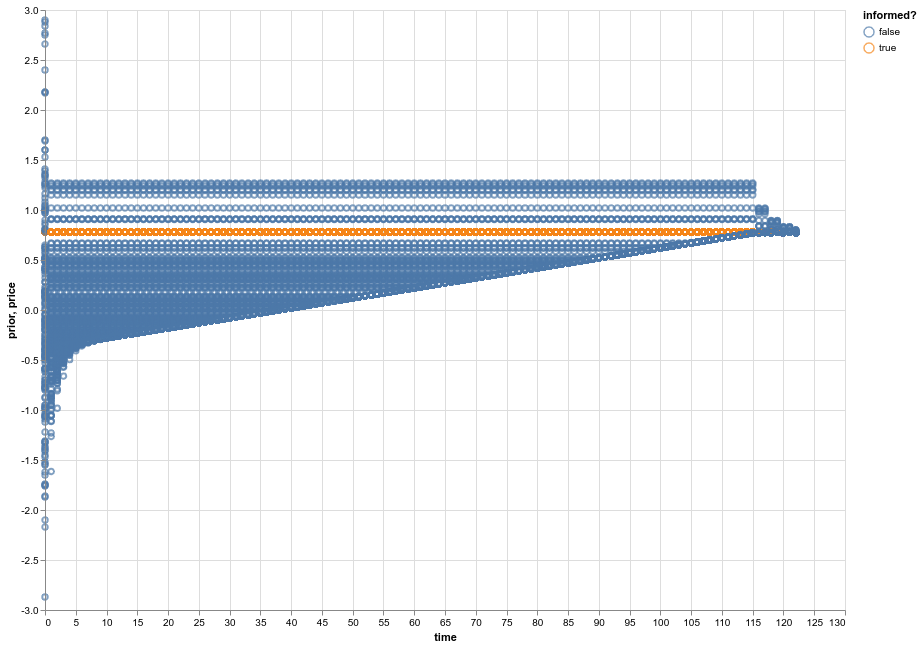
\includegraphics[width=.9\linewidth]{./plots/1-param-price.png}
\caption{\label{fig:org80c324a}
Price convergence for a market with one parameter, as in GS}
\end{figure}


\begin{figure}[htbp]
\centering
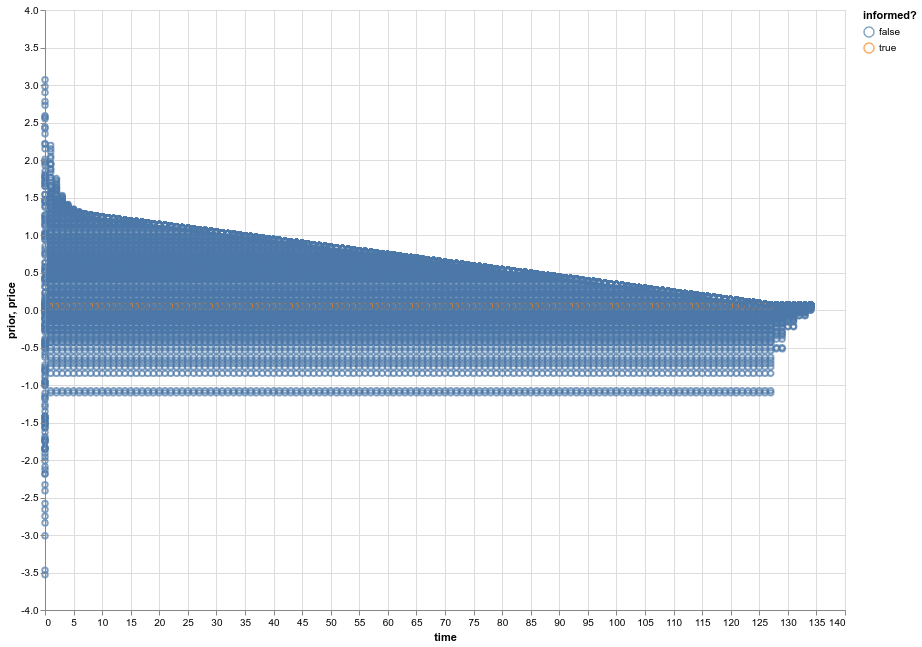
\includegraphics[width=.9\linewidth]{./plots/2-param-price.png}
\caption{\label{fig:orgbb4d8bb}
Price convergence for a market with two parameters}
\end{figure}

\begin{figure}[htbp]
\centering
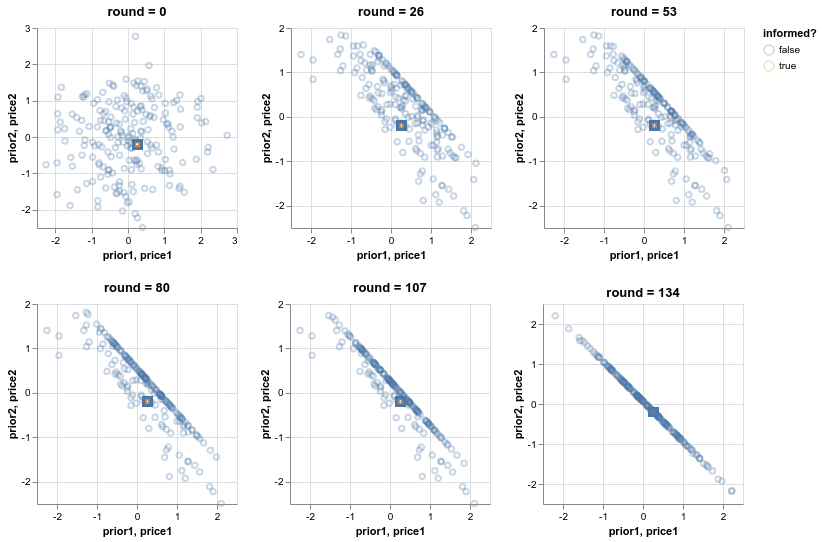
\includegraphics[width=.9\linewidth]{./plots/2-param-investors.png}
\caption{\label{fig:orge0cf8ae}
Prior updating by investors with two parameters}
\end{figure}

\begin{longtable}{|ccC{3cm}C{3cm}|}
\caption{\label{tab:org72896a6}
Sum of Squared Errors as the Number of Parameters Increases}
\\
\hline
Number of Parameters & Mean SSE & t-stat - test of difference with market size 2 & t-stat - test of difference with market size n-1\\
2 & 0.078 &  & \\
3 & 0.109 & 4.426 & 4.426\\
4 & 0.129 & 7.34 & 2.85\\
5 & 0.131 & 8.406 & 0.312\\
6 & 0.141 & 10.145 & 1.812\\
7 & 0.139 & 10.061 & -0.246\\
8 & 0.142 & 10.624 & 0.418\\
9 & 0.137 & 10.332 & -0.918\\
10 & 0.15 & 12.112 & 2.74\\
\hline
\end{longtable}
\end{document}
